\documentclass{beamer}

\usepackage[english]{babel}
\usepackage[utf8]{inputenc}
\usepackage{float} % per posizionare le figure float opzione H
\usepackage{amsfonts}
\usepackage{amsmath}
\usepackage{amsthm}
\usepackage{amssymb}
\usepackage[ruled,linesnumbered]{algorithm2e} % per gli algoritmi in pseudocodice
\usepackage{listings} % per inserire il codice in C
\usepackage{longtable}
\usepackage{booktabs}
\usepackage{graphicx} % to include images
\usepackage{xspace}
\usepackage{hyperref}
\usepackage[]{xcolor}
% \usepackage{rotating}
\usepackage{dirtree}
\usepackage[hang,small,sc]{caption}

% Codici %
\renewcommand\lstlistingname{Listing}
\renewcommand\lstlistlistingname{Listings}
% END Codici %

% ALIAS %
\newcommand{\dt}{TosKer\xspace}

%TOSKER MODULES
\newcommand{\mdeployer}{\emph{Orchestrator}\xspace}
\newcommand{\mparser}{\emph{TOSCA utility}\xspace}
\newcommand{\msoftware}{\emph{Software manager}\xspace}
\newcommand{\mcontainer}{\emph{Container manager}\xspace}
\newcommand{\mvolume}{\emph{Volume manager}\xspace}
\newcommand{\mdocker}{\emph{Docker interface}\xspace}
\newcommand{\mmanager}{\emph{Managers}\xspace}

%TOSKER TYPES
\newcommand{\tpersistent}{\emph{tosker.\-nodes.\-Container.\-Executable}\xspace}
\newcommand{\tcontainer}{\emph{tosker.\-nodes.\-Container}\xspace}
\newcommand{\tvolume}{\emph{tosker.\-nodes.\-Volume}\xspace}
\newcommand{\timage}{\emph{tosker.\-artifacts.\-Image}\xspace}
\newcommand{\tdockerfile}{\emph{tosker.\-artifacts.\-Dockerfile}\xspace}
\newcommand{\tsoftware}{\emph{tosker.\-nodes.\-Software}\xspace}
% END ALIAS %

% Definition of the colours
\definecolor{codegreen}{rgb}{0,0.6,0}
\definecolor{codegray}{rgb}{0.5,0.5,0.5}
\definecolor{codepurple}{rgb}{0.58,0,0.82}
\definecolor{backcolour}{rgb}{0.95,0.95,0.92}
\definecolor{deepblue}{rgb}{0,0,0.5}
\definecolor{deepred}{rgb}{0.6,0,0}
\definecolor{deepgreen}{rgb}{0,0.5,0}

% Default fixed font does not support bold face
\DeclareFixedFont{\ttb}{T1}{txtt}{bx}{n}{10} % for bold
\DeclareFixedFont{\ttm}{T1}{txtt}{m}{n}{10}  % for normal

% LISTINGS YAML %
\newcommand\YAMLcolonstyle{\color{red}\footnotesize\mdseries}
\newcommand\YAMLkeystyle{\color{black}\footnotesize\bfseries}
\newcommand\YAMLvaluestyle{\color{blue}\footnotesize\mdseries}

\makeatletter

% here is a macro expanding to the name of the language
% (handy if you decide to change it further down the road)
\newcommand\language@yaml{yaml}

\expandafter\expandafter\expandafter\lstdefinelanguage
\expandafter{\language@yaml}
{
  keywords={true,false,null,y,n},
  keywordstyle=\color{darkgray}\bfseries,
  basicstyle=\YAMLkeystyle,                                 % assuming a key comes first
  sensitive=false,
  comment=[l]{\#},
  morecomment=[s]{/*}{*/},
  commentstyle=\color{purple}\ttfamily,
  stringstyle=\YAMLvaluestyle\ttfamily,
  moredelim=[l][\color{orange}]{\&},
  moredelim=[l][\color{magenta}]{*},
  moredelim=**[il][\YAMLcolonstyle{:}\YAMLvaluestyle]{:},   % switch to value style at :
  morestring=[b]',
  morestring=[b]",
  literate =    {---}{{\ProcessThreeDashes}}3
                {>}{{\textcolor{red}\textgreater}}1
                {|}{{\textcolor{red}\textbar}}1
                {\ -\ }{{\mdseries\ -\ }}3,
}

% switch to key style at EOL
\lst@AddToHook{EveryLine}{\ifx\lst@language\language@yaml\YAMLkeystyle\fi}
\makeatother

\newcommand\ProcessThreeDashes{\llap{\color{cyan}\mdseries-{-}-}}

\lstdefinestyle{TOSCA}{
  captionpos=t,
  % abovecaptionskip=0.8\baselineskip,
  belowcaptionskip=0.8\baselineskip,
  keepspaces=true,
  numbersep=5pt,
  xleftmargin=\parindent,
  language=yaml,
  % basicstyle=\ttm,
  basicstyle=\footnotesize\ttfamily,
  commentstyle=\itshape\color{purple!40!black},
  numberstyle=\tiny\color{codegray},
  numbers=left,
  frame=tb,
}
%% END LISTINGS YAML %%


%% LISTING PYTHON %%
\lstdefinestyle{mystyle}{
    % % backgroundcolor=\color{backcolour},
    % commentstyle=\color{codegreen},
    % keywordstyle=\ttb\color{deepblue},
    % numberstyle=\tiny\color{codegray},
    % stringstyle=\color{codepurple},
    % basicstyle=\ttm,
    % breakatwhitespace=false,
    % breaklines=true,
    % keepspaces=true,
    % numbers=left,
    % numbersep=5pt,
    % showspaces=false,
    % showstringspaces=false,
    % showtabs=false,
    % tabsize=2,
    % language=Python
    captionpos=t,
    belowcaptionskip=0.8\baselineskip,
    % abovecaptionskip=1\baselineskip,
    breaklines=true,
    language=Python,
    basicstyle=\ttm,
    otherkeywords={self},             % Add keywords here
    keywordstyle=\ttb\color{deepblue},
    emph={MyClass,__init__},          % Custom highlighting
    emphstyle=\ttb\color{deepred},    % Custom highlighting style
    stringstyle=\color{deepgreen},
    commentstyle=\color{codegray},
    numberstyle=\tiny\color{codegray},
    numbers=left,
    frame=tb,                         % Any extra options here
    showstringspaces=false            %
}

%% END LISTING PYTHON %%


\usepackage{graphicx}
\usepackage{caption}
\usepackage{subcaption}

% \usepackage[backend=bibtex, sorting=nty, style=numeric]{biblatex}
% \addbibresource{../references.bib}

\usetheme{Frankfurt}
\usecolortheme{whale}
% #3778C6
\definecolor{myblue1}{RGB}{55,120,198}
\definecolor{myblue2}{RGB}{37,78,136}
\definecolor{myblue3}{RGB}{0,20,137}
% \definecolor{white}{RGB}{255,255,255}
% \definecolor{black}{RGB}{0,0,0}


\setbeamercolor*{frametitle}{fg=white,bg=myblue2}
\setbeamercolor*{title}{fg=white,bg=myblue2}
\setbeamercolor*{structure}{fg=myblue2}


\title[About Beamer] %optional
{Orchestrating applications with\\ TOSCA and Docker}

% \subtitle{A short story}

\author[Candidate: Rinaldi] % (optional, for multiple authors)
{Luca Rinaldi}

\institute[] % (optional)
{
  {\small
  MSc in Computer Science and Networking
  \\
  University of Pisa and Sant'Anna School of Advanced Studies}
  \\
  A.Y. 2015/2016
}

% \logo{\includegraphics[height=1.5cm]{../thesis/style/logo.png}}

\date[2016] % (optional)
{
  \small
  Supervisors: Antonio Brogi, Jacopo Soldani
}

% \AtBeginSubsection[]
% {
% \begin{frame}{Table of Contents}
% \tableofcontents[
%   currentsection,
%   currentsubsection,
%   sectionstyle=show/shaded,
%   subsectionstyle=show/shaded
% ]
% \end{frame}
% }
\AtBeginSection[]{
  \begin{frame}{Table of Contents}
    \tableofcontents[currentsection]
  \end{frame}
}

\begin{document}
\begin{frame}
  \maketitle
\end{frame}

% \begin{frame}{Table of Contents}
%   \tableofcontents
% \end{frame}

\section{Context and motivations}\subsection{}
  % \begin{frame}{Context(I)}
  %   % The possibility of automating the deployment of (complex) applications over heterogeneous infrastructures, by taking into account both application requirements and infrastructure constraints, is receiving increasing attention.
  %   \begin{figure}
  %     \includegraphics[width=0.7\textwidth]{img/cloud-computing.png}
  %   \end{figure}
  % \end{frame}

  \begin{frame}[t]{Context: Managing composite cloud applications}
    \vspace*{-2.8em}
    \begin{columns}[T]
      \begin{column}{.3\textwidth}
        \centering
        \onslide<1->{
          \begin{figure}
            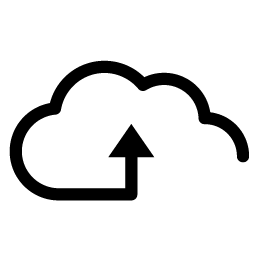
\includegraphics[width=\textwidth]{img/deployment_black.png}
          \end{figure}
          \vspace*{-2em}
          {\Huge ?}
        }
      \end{column}
    \end{columns}

    \vspace*{-2.5em}
    \begin{columns}[b]
      \begin{column}{.3\textwidth}
        \centering
        \onslide<2->{
          \begin{figure}
            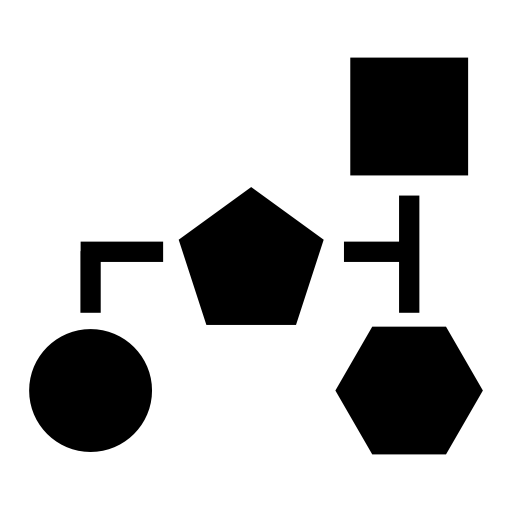
\includegraphics[width=0.7\textwidth]{img/application.png}
          \end{figure}
          {\large Application specification}
        }
      \end{column}
      \begin{column}{.3\textwidth}

      \end{column}
      \begin{column}{.3\textwidth}
        \centering
        \onslide<3->{
          \begin{figure}
            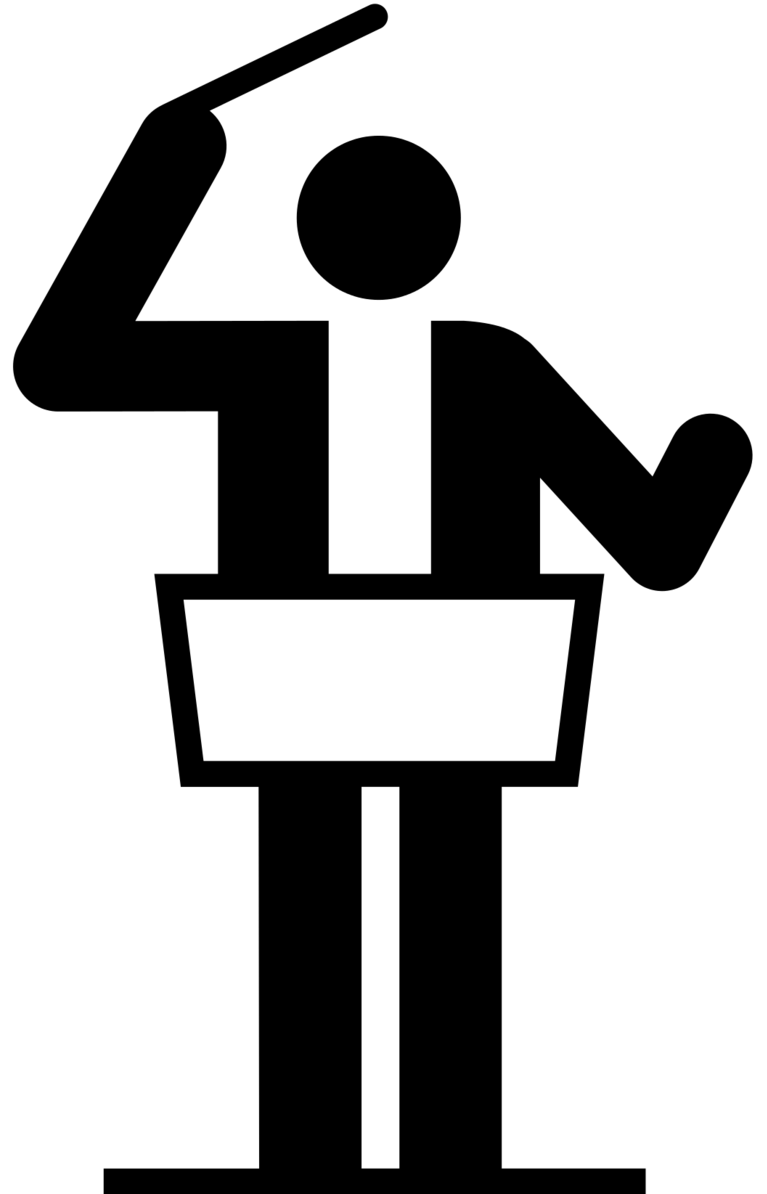
\includegraphics[width=0.6\textwidth]{img/orchestrate.png}
          \end{figure}
          {\large Application orchestration}
        }
      \end{column}
    \end{columns}
    % Application orchestration
  \end{frame}

  \begin{frame}{Two orthogonal approaches}
    \begin{columns}[b]
      \begin{column}{0.5\textwidth}
        \centering
        \onslide<1->{
          \begin{figure}
            
\includegraphics[width=0.7\textwidth]{img/oasis_logo.jpg}
          \end{figure}
          {\Large OASIS TOSCA}
        }
      \end{column}
      \begin{column}{0.5\textwidth}
        \centering
        \onslide<2>{
          \begin{figure}
            
\includegraphics[width=0.8\textwidth]{img/docker.png}
          \end{figure}
          {\Large Docker}
        }
      \end{column}
    \end{columns}
    % \begin{columns}[onlytextwidth]
    %   \begin{column}{0.5\textwidth}
    %       TOSCA is an OASIS standard that provides a YAML-based modelling language for specifying portable cloud applications, and for automating their deployment and management.
    %   \end{column}
    %   \begin{column}{0.5\textwidth}
    %       Docker is an open source platform for building, shipping, and running software components, together with their dependencies, in lightweight virtual environments, called containers.
    %   \end{column}
    % \end{columns}
  \end{frame}

  \begin{frame}{Pro and cons of TOSCA and Docker}
    \begin{columns}[T]
      \begin{column}{.5\textwidth}
        \centering
        % \begin{block}{TOSCA}
          {\Large TOSCA}
          \medskip
          \begin{itemize}
            \item[\textcolor{green}{\textbf{+}}] Well-documented standard
            \item[\textcolor{green}{\textbf{+}}] Application orchestration\pause\medskip
            \item[\textcolor{red}{\textbf{--}}] Too verbose
            \item[\textcolor{red}{\textbf{--}}] Lack of engines\pause
          \end{itemize}
        % \end{block}
      \end{column}
      \begin{column}{.5\textwidth}
        \centering
        {\Large Docker}
        \medskip
        \begin{itemize}
          \item[\textcolor{green}{\textbf{+}}] Production ready tool
          \item[\textcolor{green}{\textbf{+}}] Repository of images\pause\medskip
          \item[\textcolor{red}{\textbf{--}}] Application orchestration
          \item[\textcolor{red}{\textbf{--}}] ``Only containers''
        \end{itemize}
      \end{column}
    \end{columns}
  \end{frame}

  \begin{frame}{Objective}
    The objective of this thesis was to identify and develop a solution that takes the best of TOSCA and Docker.
    \begin{block}{Main objective}
      Design and prototype an orchestration engine capable of deploying multi-components applications.
      \begin{itemize}
        \item It inputs applications specified in TOSCA YAML
        \item It automatically manages applications by exploiting Docker
      \end{itemize}
    \end{block}
  \end{frame}

  \begin{frame}[t]{State of the art}
    %  Indeed, to the best of our knowledge, current solutions either provide a support for TOSCA or permit orchestrating multi-component Docker applications.
    \begin{columns}[T]
      \begin{column}{0.4\textwidth}
        \centering
        \onslide<1->{
          {\large\textbf{TOSCA orchestrator}}
          \begin{figure}
            
\includegraphics[width=\textwidth]{img/opentosca.jpg}
          \end{figure}
          \begin{figure}
            
\includegraphics[width=0.6\textwidth]{img/alien4cloud.png}
          \end{figure}
        }
      \end{column}
      \begin{column}{0.4\textwidth}
        \centering
        \onslide<3>{
          % {\large\textbf{Somethings in between}}
          \begin{figure}
            
\includegraphics[width=\textwidth]{img/claudify.png}
          \end{figure}
          \begin{figure}
            
\includegraphics[width=0.9\textwidth]{img/brooklyn.png}
          \end{figure}
        }
      \end{column}
      \begin{column}{0.4\textwidth}
        \centering
        \onslide<2->{
          {\large\textbf{Docker orchestrator}}
          \vspace*{-1.1em}
          \begin{figure}
            
\includegraphics[width=0.68\textwidth]{img/kubernetes.png}
          \end{figure}
          \vspace*{-1.7em}
          \begin{figure}
            
\includegraphics[width=0.75\textwidth]{img/mesos_crop.png}
          \end{figure}
          \vspace*{-1.7em}
          \begin{figure}
            
\includegraphics[width=0.68\textwidth]{img/docker_compose.png}
          \end{figure}
        }
      \end{column}
    \end{columns}
  \end{frame}


\section{Our solution: \dt}
\subsection*{Design}
  % \begin{frame}{}%{\dt}
  %
  %    \begin{center}
  %      {\Huge\textbf{\dt}}
  %    \end{center}
  %    \bigskip
  %    An orchestration engine capable of deploying, on top of Docker, applications described in TOSCA YAML.
  %
  %   %  \dt inputs a TOSCA description of a multi-component application, where some components are Docker containers and Docker volumes, and automatically deploys and orchestrates it using the Docker engine.
  % \end{frame}

  \begin{frame}{Describing applications in \dt}
    \begin{itemize}
      \item Applications are specified as a composition of the following components:\begin{itemize}
          \item \small\emph{Docker containers} {\tiny\texttt{tosker.nodes.Container, tosker.nodes.Container.Executable}}
          \item \small\emph{Docker volumes} {\tiny\texttt{tosker.nodes.Volume}}
          \item \small\emph{Software} {\tiny\texttt{tosker.nodes.Software}}
        \end{itemize}\pause
      \item There can be the following relationships between components:\begin{itemize}
          \item \small\emph{hosted on} {\tiny\texttt{tosca.relationships.HostedOn}}
          \item \small\emph{connected to} {\tiny\texttt{tosca.relationships.ConnectsTo}}
          \item \small\emph{attached to} {\tiny\texttt{tosca.relationships.AttachesTo}}
          \item \small\emph{depending on} {\tiny\texttt{tosca.relationships.DependsOn}}
        \end{itemize}
        % \pause
        % \item Each application must meet some constrains, e.g.,
        %     \begin{itemize}
        %       \item \small A \emph{software} must be ``\emph{hosted on}'' another \emph{software} or a \emph{Docker container}
        %       \item \small A \emph{Docker container} and \emph{Docker volume} cannot be ``\emph{hosted on}'' other components
        %       \item \small Only \emph{Docker containers} can be ``\emph{attached to}'' \emph{Docker volumes}
        %     \end{itemize}
    \end{itemize}
  \end{frame}

  \begin{frame}{Use case}
    \begin{figure}
      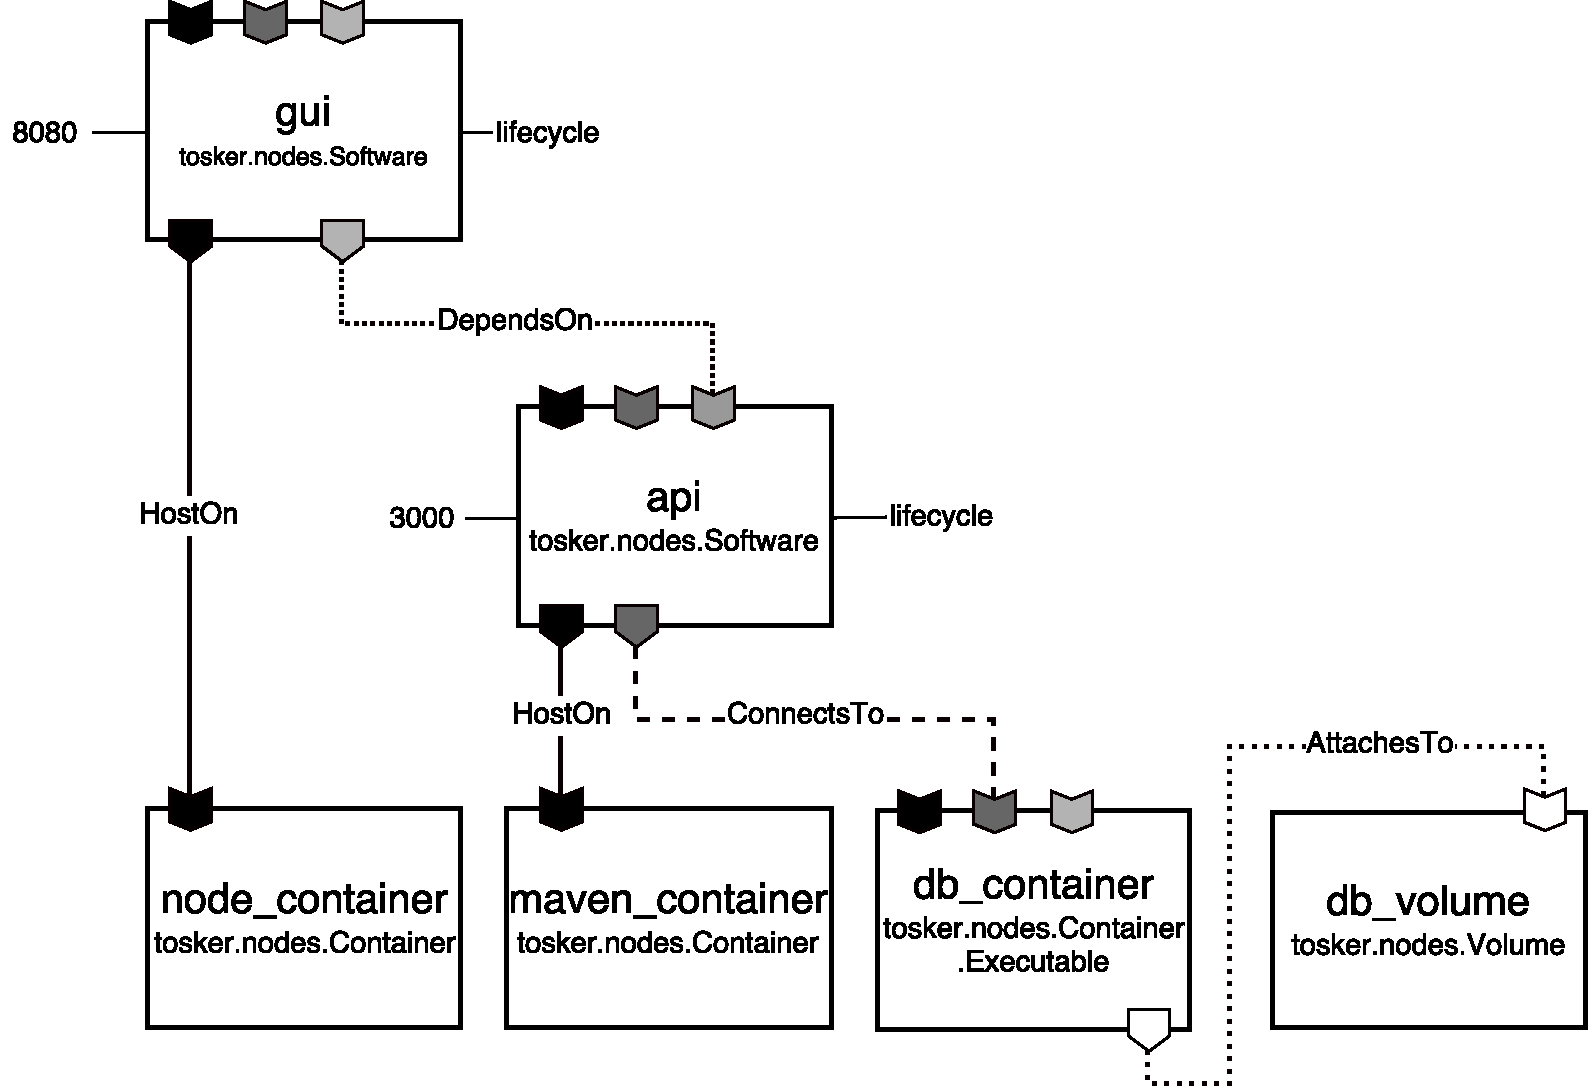
\includegraphics[width=\textwidth]{../thesis/img/thoughts_graph.pdf}
    \end{figure}
  \end{frame}

  \begin{frame}{Architecture of \dt}
    \begin{figure}
        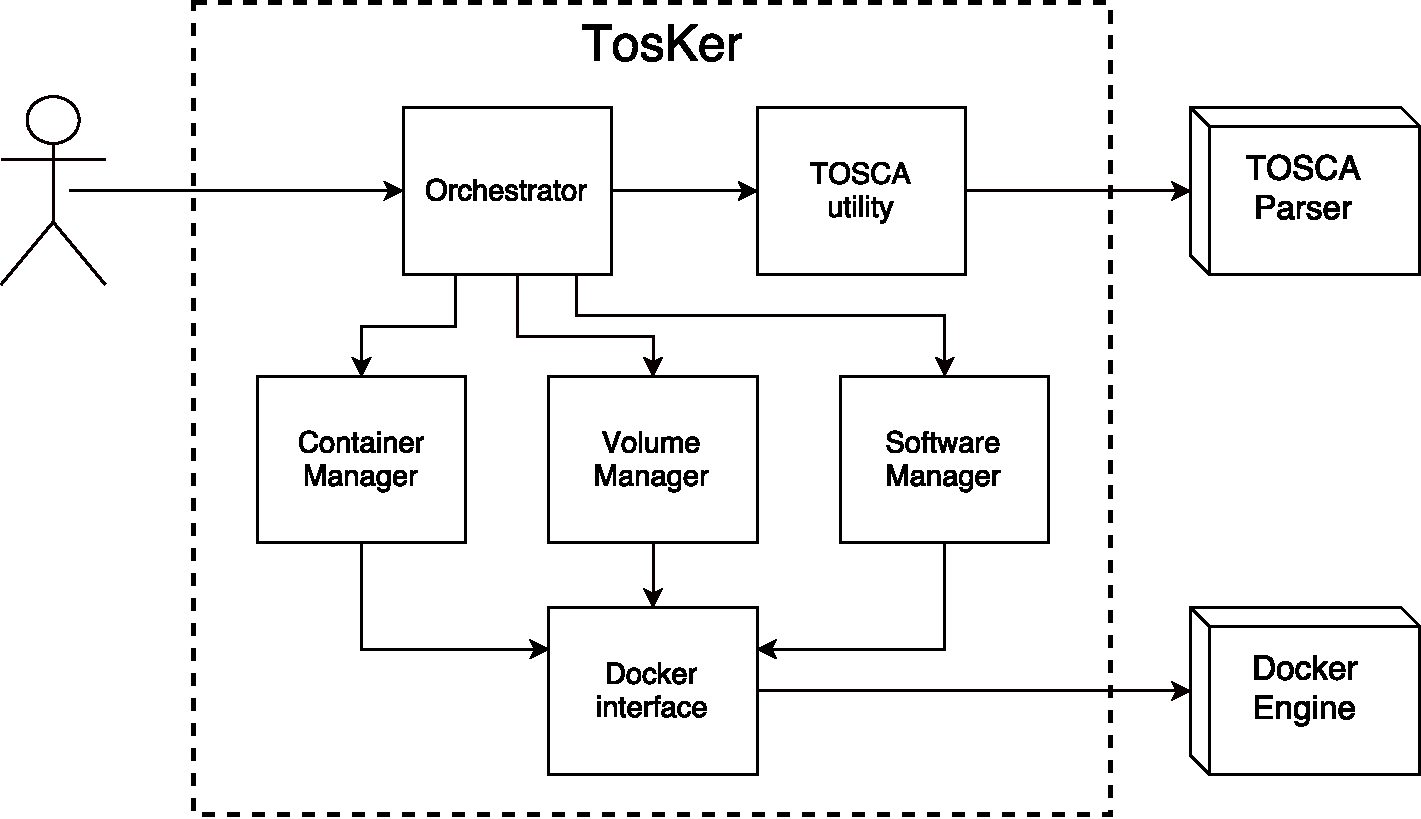
\includegraphics[width=0.9\textwidth]{../thesis/img/tosker_design.pdf}
      \end{figure}
  \end{frame}

  \begin{frame}[t]{How \dt orchestrates applications}
    % \vspace*{-.5em}
    \only<1>{
      \begin{figure}
        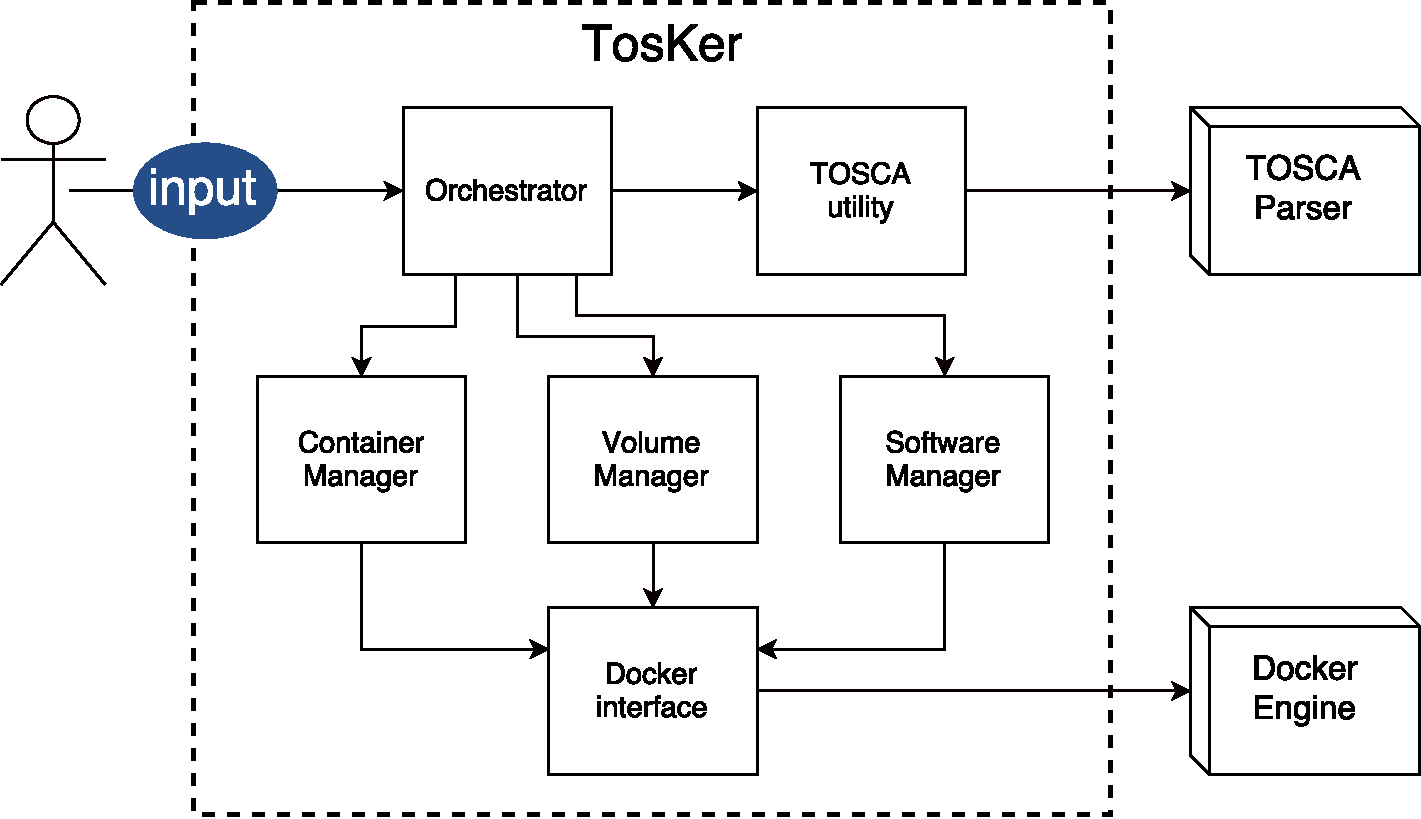
\includegraphics[width=0.8\textwidth]{img/tosker_design_input.pdf}
      \end{figure}
      The input of \dt is
      \begin{itemize}
        \item a TOSCA application specified using \dt types, and
        \item management operation(s) to perform.
      \end{itemize}
    }
    \only<2>{
      \begin{figure}
        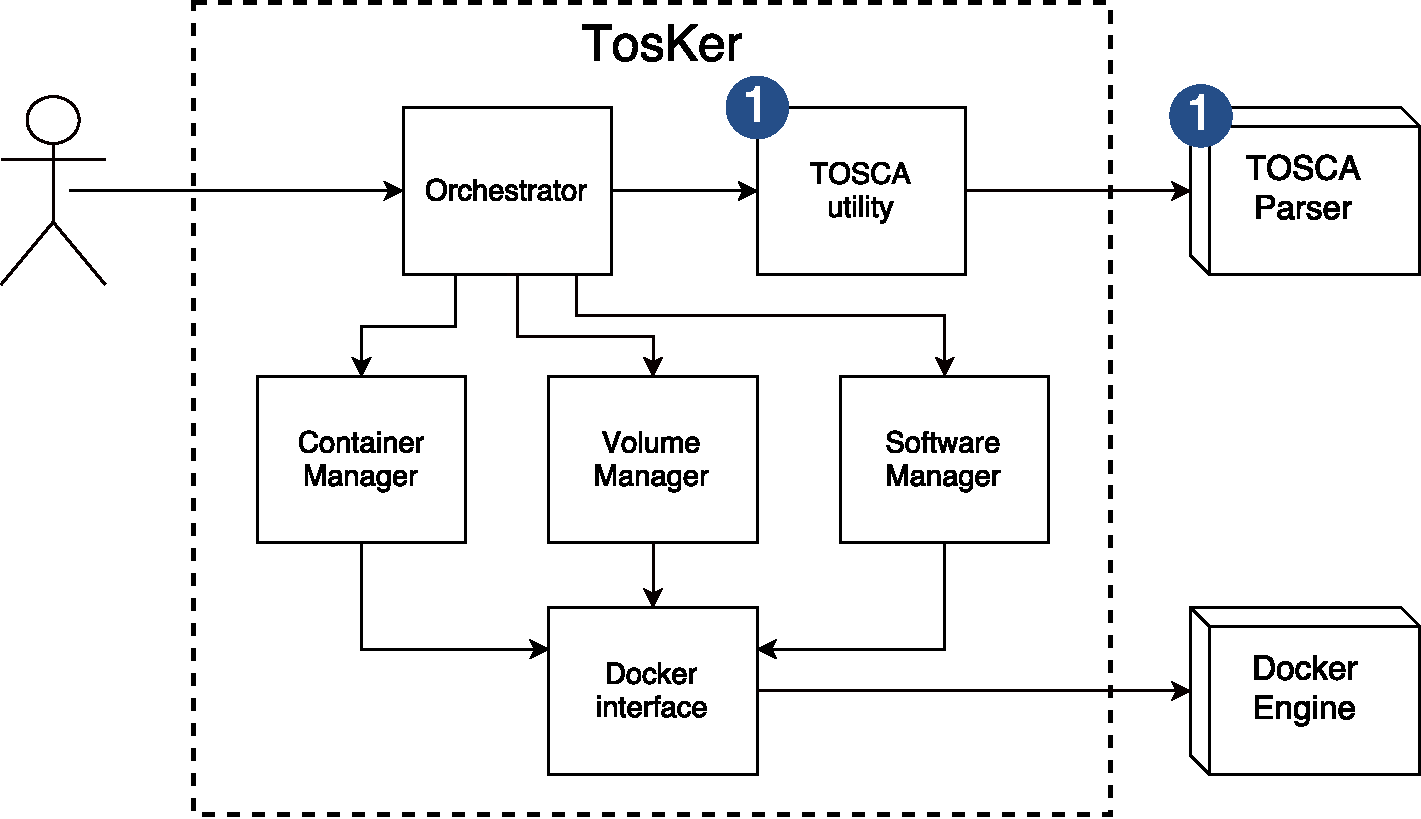
\includegraphics[width=.8\textwidth]{img/tosker_design_1.pdf}
      \end{figure}
      \vspace*{-.5em}
      \dt
      \begin{itemize}
        \item parses and validates the TOSCA application, and
        % \item create an internal representation of the application
        \item executes a topological sorting algorithm.
      \end{itemize}
    }
    \only<3>{
      \begin{figure}
        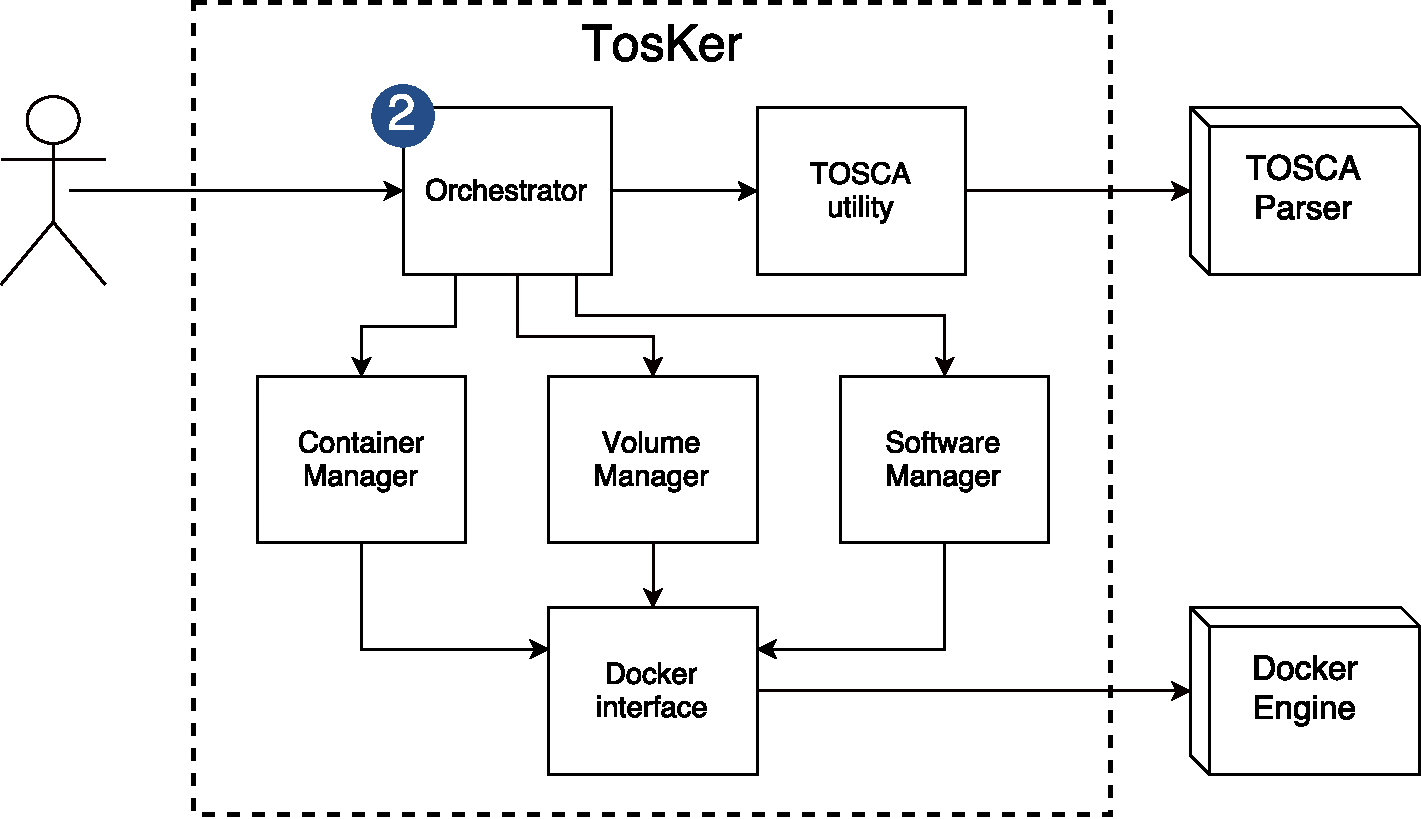
\includegraphics[width=.8\textwidth]{img/tosker_design_2.pdf}
      \end{figure}
      \vspace*{-.5em}
      \dt %exploits the (topologically sorted) application to orchestrate it:
      \begin{itemize}
        \item scans the sorted application topology, and
        \item for each component, it calls a specific operation (e.g., create)
      \end{itemize}
    }
    \only<4>{
      \begin{figure}
        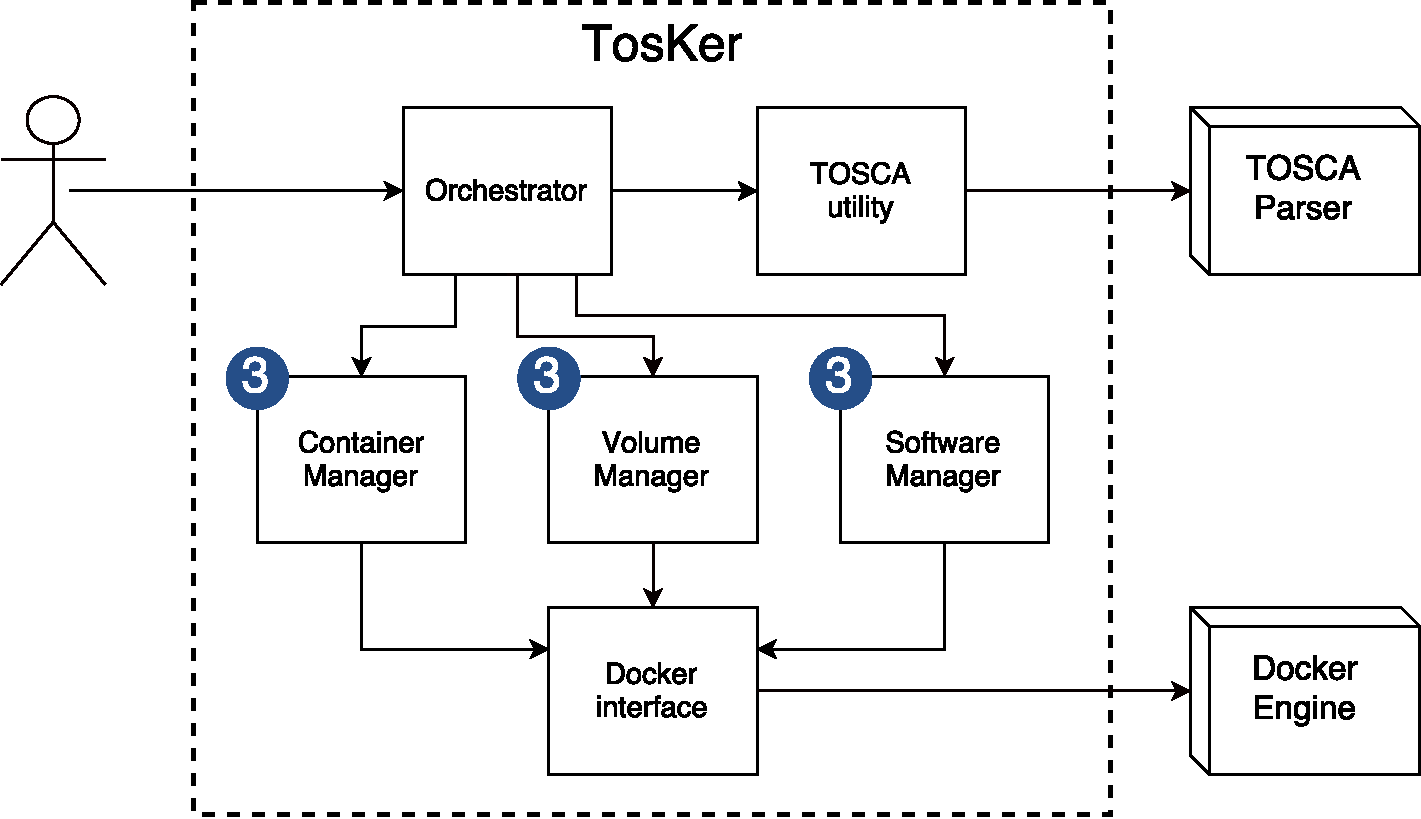
\includegraphics[width=.8\textwidth]{img/tosker_design_3.pdf}
      \end{figure}
      Each manager is in charge of implementing/executing the invoked operation on a component...
    }
    \only<5>{
      \begin{figure}
        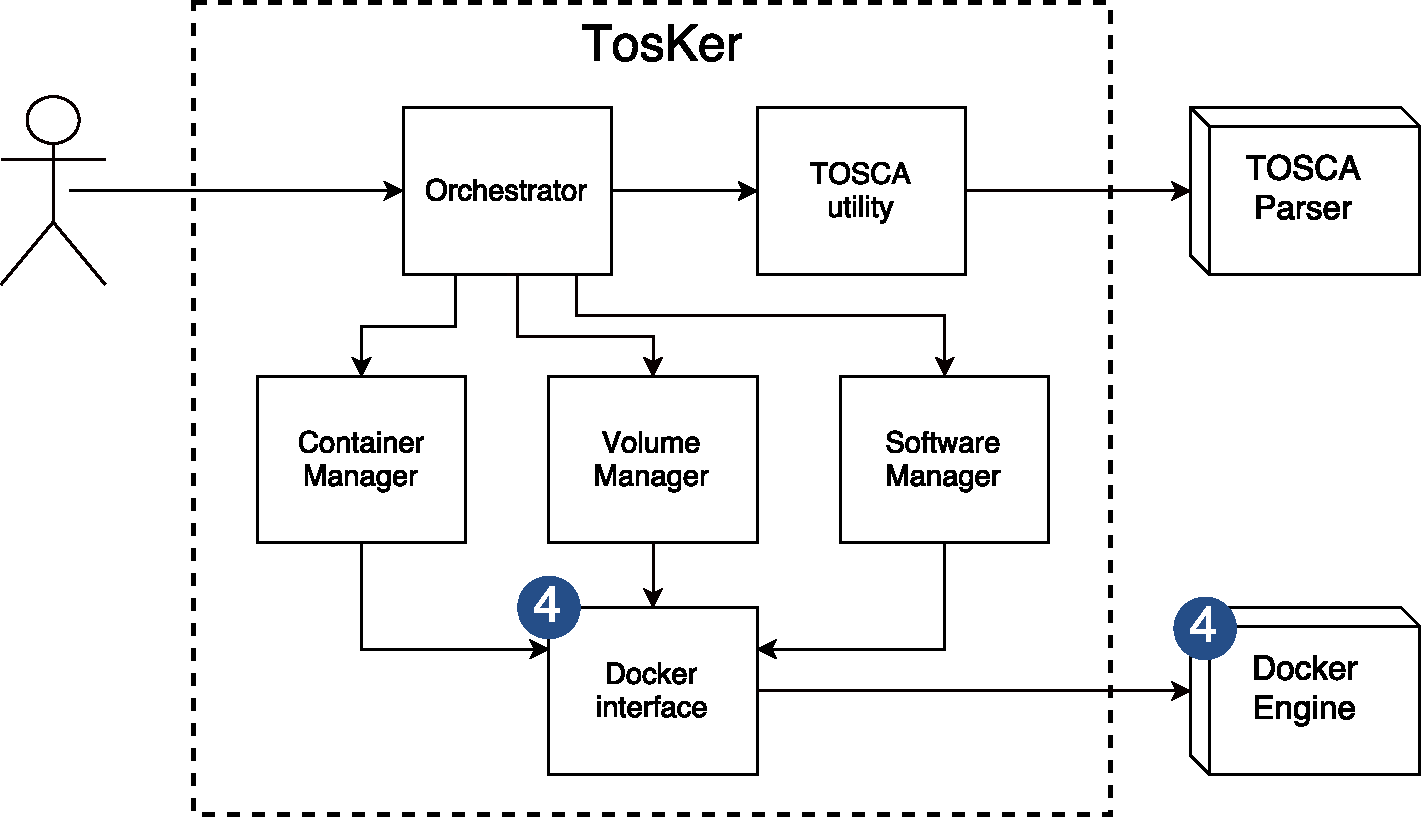
\includegraphics[width=.8\textwidth]{img/tosker_design_4.pdf}
      \end{figure}
      ...by properly invoking the Docker engine (through the Docker interface)
    }
  \end{frame}


\subsection*{Prototype}
  \begin{frame}{Implementation of \dt}
    \begin{columns}[b]
      \begin{column}{.3\textwidth}
        \centering
        \onslide<1->{
          \begin{figure}
            
\includegraphics[width=.6\textwidth]{img/python.png}
          \end{figure}
          {\large Python}
        }
      \end{column}
      \begin{column}{.3\textwidth}
        \centering
        \onslide<2->{
          \begin{figure}
            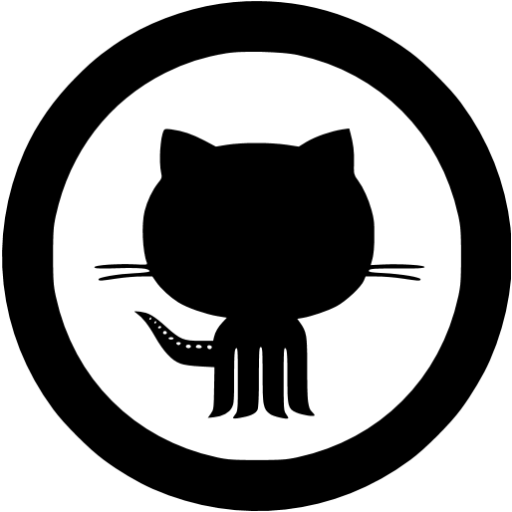
\includegraphics[width=.6\textwidth]{img/github.png}
          \end{figure}
          {\large GitHub}
        }
      \end{column}
      \begin{column}{.3\textwidth}
        \centering
        \onslide<2>{
          \begin{figure}
            
\includegraphics[width=.6\textwidth]{img/mit.png}
          \end{figure}
          {\large MIT Licence}
        }
      \end{column}
    \end{columns}
      \vspace{20pt}
      \begin{itemize}
        \item \onslide<1->{
          \small\textbf{PyPI}: \href{https://pypi.python.org/pypi/tosKer}{https://pypi.python.org/pypi/tosKer}\\
          \indent\indent\texttt{pip install tosker}\vspace{10pt}
        }
        \item \onslide<2>{
          \small\textbf{GitHub}: \href{https://github.com/di-unipi-socc/tosKer}{https://github.com/di-unipi-socc/tosKer}
        }
      \end{itemize}
    % \dt is implemented using \textbf{Python}
  %   \dt exploits the following open-source library:
  %   \begin{itemize}
  %     \item Docker-py
  %     \item Tosca-parser
  %   \end{itemize}
  \end{frame}

  \begin{frame}[containsverbatim]{Usage of \dt command-line}
    % \begin{columns}
    %   \begin{column}{\paperwidth}
    %     \centering
        \begin{lstlisting}[
          basicstyle=\ttfamily\scriptsize,
          language=sh,
          breaklines=true
        ]
tosker FILE COMMANDS... [OPTIONS] [INPUTS]
tosker -h|--help
tosker -v|--version

FILE: TOSCA YAML file or CSAR file

COMMANDS:
  create   Create application components
  start    Start applications components
  stop     Stop application components
  delete   Delete application components (except volumes)

OPTIONS:
  -h --help      Print usage
  -v --version   Print version
  -q --quiet     Enable quiet mode
  --debug        Enable debugging mode (override quiet mode)

INPUTS: provide TOSCA inputs (syntax: --NAME VALUE)
        \end{lstlisting}
    %   \end{column}
    % \end{columns}
  \end{frame}

  \begin{frame}
    \centering
    % \only<1>{\Huge DEMO}
    % \only<2>{
    \Huge VIDEO-DEMO
    % }
  \end{frame}


\section{Conclusions and future work}\subsection*{}
  \begin{frame}{Conclusions and future work}%
    %The objective of this thesis was to design and prototype \dt an orchestration engine, which
    We have presented \dt, an orchestration engine, which
    \begin{itemize}
      \item extends TOSCA by providing a Docker-based orchestration engine for TOSCA application, and
      \item extends Docker by adding the capability of orchestrating software components together with Docker containers/volumes\pause
    \end{itemize}
    % \begin{itemize}
    %   \item Approach the problem of automatically deploying and managing of applications\pause
    %   \item Study a solution to exploit the advantages of TOSCA and Docker\pause
    %   \item Design and prototype \dt, the first orchestrator engine that manage software components and Docker components together.\pause
    % \end{itemize}
    \medskip
    {\large Future work}
    \begin{itemize}
      \item Support cluster of workstations and external cloud services\pause
      \item Automatically determine the Docker containers needed to effectively run an application\pause
      \item Integrate \dt with fault-aware management protocols
    \end{itemize}
  \end{frame}

  \begin{frame}
    \centering
    \Huge Thank You \\
    \bigskip
    \LARGE Q\&A
  \end{frame}

  % \begin{frame}{Tests Coverage}
  %   To validate \dt we developed \textbf{4 examples} and \textbf{12 units tests}.
  %   \begin{table}
  %   \centering
  %   \footnotesize
  %   % \caption{Coverage of the test executed on \dt}
  %   \label{coverage}
  %   % \rotatebox{90}{
  %     \begin{tabular}{lllll}
  %     \hline
  %     Module                                & statements & missing & coverage \\
  %     \hline
  %     tosker/graph/nodes.py                 & 94         & 9       & 90\%     \\
  %     tosker/graph/template.py              & 20         & 1       & 95\%     \\
  %     tosker/managers/container\_manager.py & 31         & 2       & 94\%     \\
  %     tosker/managers/software\_manager.py  & 68         & 4       & 94\%     \\
  %     tosker/managers/volume\_manager.py    & 12         & 2       & 83\%     \\
  %     tosker/tosca\_utility.py              & 211        & 16      & 92\%     \\
  %     tosker/docker\_interface.py           & 169        & 19      & 89\%     \\
  %     tosker/orchestrator.py                & 94         & 17      & 82\%     \\
  %     tosker/helper.py                      & 69         & 38      & 45\%     \\
  %     tosker/shell.py                       & 72         & 72      & 0\%      \\
  %     \hline
  %     Total                                 & 841        & 180     & 79\%     \\
  %     \hline
  %     \end{tabular}
  %   % }
  %   \end{table}
  % \end{frame}

  % \begin{frame}[c]{\dt node types}
  %   % \begin{columns}[onlytextwidth]
  %   %  \begin{column}{0.5\textwidth}
  %     %  \centering
  %      \begin{itemize}
  %        \item \tcontainer
  %        \item \tpersistent
  %        \item \tvolume
  %        \item \tsoftware
  %        \item \tdockerfile
  %        \item \timage
  %      \end{itemize}
  % %    \end{column}
  % %    \begin{column}{0.5\textwidth}
  % %      \centering
  % %      \only<1>{
  % %        \begin{figure}[h]
  % %         \includegraphics[width=0.7\textwidth]{../thesis/img/tosker_types_container.png}
  % %        \end{figure}
  % %      }
  % %     %  \addtocounter{figure}{1}
  % %      \only<2>{
  % %        \begin{figure}[h]
  % %          \includegraphics[width=\textwidth]{../thesis/img/tosker_types_executable.png}
  % %        \end{figure}
  % %      }
  % %      \only<3>{
  % %        \begin{figure}[h]
  % %          \includegraphics[width=\textwidth]{../thesis/img/tosker_types_volume.png}
  % %        \end{figure}
  % %      }
  % %      \only<4>{
  % %        \begin{figure}[h]
  % %          \includegraphics[width=0.9\textwidth]{../thesis/img/tosker_types_software.png}
  % %        \end{figure}
  % %      }
  % %    \end{column}
  % %  \end{columns}
  % \end{frame}
\end{document}
